% All the following setup code was written by Brian Snider, Computer Science and Information Systems professor at George Fox University.

\documentclass[10pt]{exam}

\usepackage[T1]{fontenc}
\usepackage{amsmath}
\usepackage{listings}
\usepackage{tikz}
\usepackage[simplified]{pgf-umlcd}
%\usepackage{ulem}
\usepackage{url}


% listings:  format code samples
\lstset{
  language=Java,
  basicstyle=\small\ttfamily,
  commentstyle=\ttfamily,
  columns=flexible,
  breaklines=true,
  breakatwhitespace=true,
  keepspaces=true,
}

% pgf-umlcd:  use guillemets for interfaces & abstract classes
\renewenvironment{interface}[3][]{\begin{classAndInterfaceCommon}{#1}{#2}{#3}}{%
  \calcuateNumberOfParts{}
  \node[this umlcd style, anchor=north] (\umlcdClassName) at (\umlcdClassPos) {%
    \footnotesize\guillemotleft\,interface\,\guillemotright\normalsize \\ \textbf{\umlcdClassName}
    \insertAttributesAndOperations{}
  };
  \end{classAndInterfaceCommon}
}
\renewenvironment{abstractclass}[3][]{\begin{classAndInterfaceCommon}{#1}{#2}{#3}}{%
  \calcuateNumberOfParts{}
  \node[this umlcd style, anchor=north] (\umlcdClassName) at (\umlcdClassPos) {%
    \footnotesize\guillemotleft\,abstract\,\guillemotright\normalsize \\ \textbf{\umlcdClassName}
    \insertAttributesAndOperations{}
  };
  \end{classAndInterfaceCommon}
}

% pgf-umlcd:  template parameters
\tikzset{
  template parameter/.style={
    append after command={
      node [draw, densely dashed, umlcolor, font=\ttfamily] at (\tikzlastnode.north east) {\footnotesize#1\normalsize}
    }
  }
}

% pgf-umlcd:  inner class associations
\usetikzlibrary{arrows.meta}
\pgfdeclarearrow{
  name=Contains,
  parameters={\the\pgfarrowlength},
  setup code={
   \pgfarrowssettipend{0pt}
   \pgfarrowssetlineend{-\pgfarrowlength}
   \pgfarrowlinewidth=\pgflinewidth
   \pgfarrowssavethe\pgfarrowlength
  },
  drawing code={
   \pgfpathcircle{\pgfpoint{-0.5\pgfarrowlength}{0pt}}{0.5\pgfarrowlength}
   \pgfpathmoveto{\pgfpoint{0.0\pgfarrowlength}{0.0\pgfarrowlength}}
   \pgfpathlineto{\pgfpoint{-1.0\pgfarrowlength}{0.0\pgfarrowlength}}
   \pgfpathmoveto{\pgfpoint{-0.5\pgfarrowlength}{0.5\pgfarrowlength}}
   \pgfpathlineto{\pgfpoint{-0.5\pgfarrowlength}{-0.5\pgfarrowlength}}
   \pgfusepathqstroke
  },
  defaults={length=7pt}
}
\tikzstyle{umlcd style associationinner}=[<-,>=Contains, umlcolor, >=angle 90]
\newcommand{\associationinner}[6]{
  \draw [<-,>=Contains] (#1) -- (#4)
  node[near start, above]{#2}
  node[near start, below]{#3}
  node[near end, above]{#5}
  node[near end, below]{#6};
}


% pgf-umlcd:  make readable for b&w printout
\renewcommand{\umltextcolor}{black}
\renewcommand{\umldrawcolor}{black}
\renewcommand{\umlfillcolor}{white}
\tikzset{every node/.append style={font=\ttfamily}}

% ulem:  set underline depth
%\renewcommand{\ULdepth}{3pt}

\begin{document}

\section*{Graph Implementation}
\subsection*{Class Diagram}

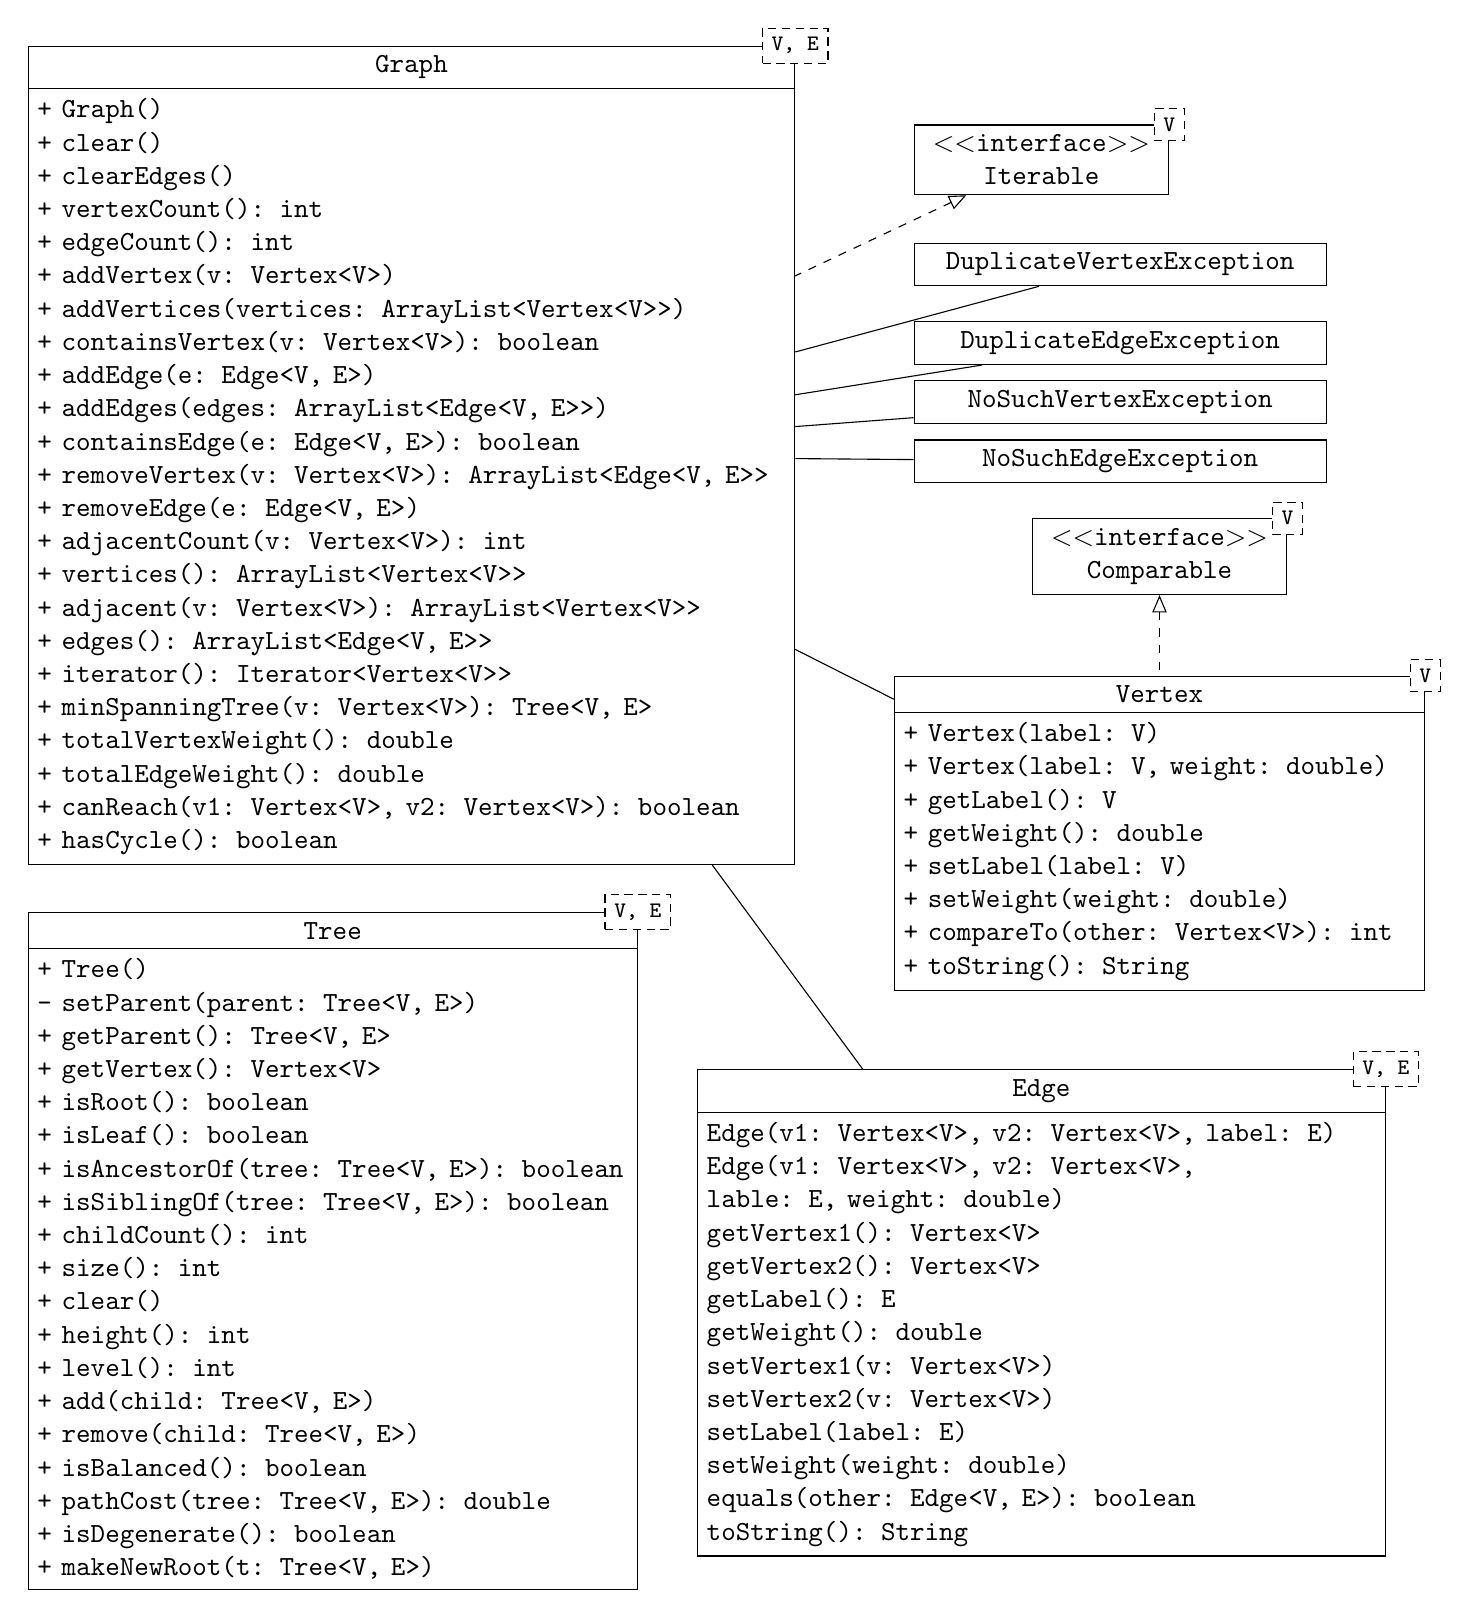
\begin{tikzpicture}

\begin{interface}[template parameter={V}, text width=3cm]{Iterable}{8,10}
%\operation[0]{+ iterator(): Iterator<T>}
\end{interface}

\begin{interface}[template parameter={V}, text width=3cm]{Comparable}{9.5,5}
%\operation[0]{+ compareTo(): int}
\end{interface}

\begin{class}[template parameter={V}, text width=6.5cm]{Vertex}{9.5,3}
  \implement{Comparable}
  \operation{+ Vertex(label: V)}
  \operation{+ Vertex(label: V, weight: double)}
  \operation{+ getLabel(): V}
  \operation{+ getWeight(): double}
  \operation{+ setLabel(label: V)}
  \operation{+ setWeight(weight: double)}
  \operation{+ compareTo(other: Vertex<V>): int}
  \operation{+ toString(): String}
\end{class}

\begin{class}[template parameter={V, E}, text width=8.5cm]{Edge}{8,-2}
  \operation{Edge(v1: Vertex<V>, v2: Vertex<V>, label: E)}
  \operation{Edge(v1: Vertex<V>, v2: Vertex<V>, lable: E, weight: double)}
  \operation{getVertex1(): Vertex<V>}
  \operation{getVertex2(): Vertex<V>}
  \operation{getLabel(): E}
  \operation{getWeight(): double}
  \operation{setVertex1(v: Vertex<V>)}
  \operation{setVertex2(v: Vertex<V>)}
  \operation{setLabel(label: E)}
  \operation{setWeight(weight: double)}
  \operation{equals(other: Edge<V, E>): boolean}
  \operation{toString(): String}
\end{class}

\begin{class}[template parameter={V, E}, text width=9.5cm]{Graph}{0,11}
  \implement{Iterable}
  \operation{+ Graph()}
  \operation{+ clear()}
  \operation{+ clearEdges()}
  \operation{+ vertexCount(): int}
  \operation{+ edgeCount(): int}
  \operation{+ addVertex(v: Vertex<V>)}
  \operation{+ addVertices(vertices: ArrayList<Vertex<V$\textup{>}$>)}
  \operation{+ containsVertex(v: Vertex<V>): boolean}
  \operation{+ addEdge(e: Edge<V, E>)}
  \operation{+ addEdges(edges: ArrayList<Edge<V, E$\textup{>}$>)}
  \operation{+ containsEdge(e: Edge<V, E>): boolean}
  \operation{+ removeVertex(v: Vertex<V>): ArrayList<Edge<V, E$\textup{>}$>}
  \operation{+ removeEdge(e: Edge<V, E>)}
  \operation{+ adjacentCount(v: Vertex<V>): int}
  \operation{+ vertices(): ArrayList<Vertex<V$\textup{>}$>}
  \operation{+ adjacent(v: Vertex<V>): ArrayList<Vertex<V$\textup{>}$>}
  \operation{+ edges(): ArrayList<Edge<V, E$\textup{>}$>}
  \operation{+ iterator(): Iterator<Vertex<V$\textup{>}$>}
  \operation{+ minSpanningTree(v: Vertex<V>): Tree<V, E>}
  \operation{+ totalVertexWeight(): double}
  \operation{+ totalEdgeWeight(): double}
  \operation{+ canReach(v1: Vertex<V>, v2: Vertex<V>): boolean}
  \operation{+ hasCycle(): boolean}
\end{class}

\begin{class}[template parameter={V, E}, text width=7.5cm]{Tree}{-1,0}
  \operation{+ Tree()}
  \operation{- setParent(parent: Tree<V, E>)}
  \operation{+ getParent(): Tree<V, E>}
  \operation{+ getVertex(): Vertex<V>}
  \operation{+ isRoot(): boolean}
  \operation{+ isLeaf(): boolean}
  \operation{+ isAncestorOf(tree: Tree<V, E>): boolean}
  \operation{+ isSiblingOf(tree: Tree<V, E>): boolean}
  \operation{+ childCount(): int}
  \operation{+ size(): int}
  \operation{+ clear()}
  \operation{+ height(): int}
  \operation{+ level(): int}
  \operation{+ add(child: Tree<V, E>)}
  \operation{+ remove(child: Tree<V, E>)}
  \operation{+ isBalanced(): boolean}
  \operation{+ pathCost(tree: Tree<V, E>): double}
  \operation{+ isDegenerate(): boolean}
  \operation{+ makeNewRoot(t: Tree<V, E>)}
\end{class}

\begin{class}[text width=5cm]{DuplicateVertexException}{9,8.5}
\end{class}

\begin{class}[text width=5cm]{DuplicateEdgeException}{9,7.5}
\end{class}

\begin{class}[text width=5cm]{NoSuchVertexException}{9,6.75}
\end{class}

\begin{class}[text width=5cm]{NoSuchEdgeException}{9,6}
\end{class}

\association{Graph}{}{}{Edge}{}{}
\association{Graph}{}{}{Vertex}{}{}
\association{Graph}{}{}{DuplicateVertexException}{}{}
\association{Graph}{}{}{DuplicateEdgeException}{}{}
\association{Graph}{}{}{NoSuchVertexException}{}{}
\association{Graph}{}{}{NoSuchEdgeException}{}{}

\end{tikzpicture}
\newpage
\section{Graph and Tree Example}
\begin{figure}[ht]
  \centering
  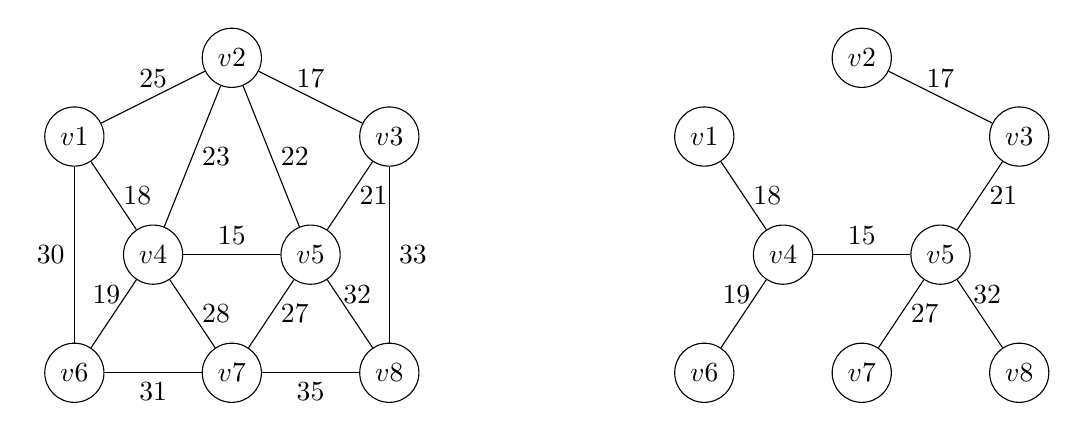
\begin{tikzpicture}
    \node[draw, shape = circle] (v1) at (0,3) {$v1$};
    \node[draw, shape = circle] (v2) at (2,4) {$v2$};
    \node[draw, shape = circle] (v3) at (4,3) {$v3$};
    \node[draw, shape = circle] (v4) at (1,1.5) {$v4$};
    \node[draw, shape = circle] (v5) at (3,1.5) {$v5$};
    \node[draw, shape = circle] (v6) at (0,0) {$v6$};
    \node[draw, shape = circle] (v7) at (2,0) {$v7$};
    \node[draw, shape = circle] (v8) at (4,0) {$v8$};

    \draw
      (v1) edge[above] node{$25$} (v2)
      (v1) edge[right] node{$18$} (v4)
      (v1) edge[left] node{$30$} (v6)
      (v4) edge[above] node{$19\ $} (v6)
      (v4) edge[right] node{$28$} (v7)
      (v4) edge[above] node{$15$} (v5)
      (v4) edge[right] node{$23$} (v2)
      (v6) edge[below] node{$31$} (v7)
      (v7) edge[right] node{$27$} (v5)
      (v7) edge[below] node{$35$} (v8)
      (v5) edge[above] node{$\ 32$} (v8)
      (v5) edge[right] node{$21$} (v3)
      (v8) edge[right] node{$33$} (v3)
      (v2) edge[right] node{$22$} (v5)
      (v2) edge[above] node{$17$} (v3);

    \node[draw, shape = circle] (v11) at (8,3) {$v1$};
    \node[draw, shape = circle] (v12) at (10,4) {$v2$};
    \node[draw, shape = circle] (v13) at (12,3) {$v3$};
    \node[draw, shape = circle] (v14) at (9,1.5) {$v4$};
    \node[draw, shape = circle] (v15) at (11,1.5) {$v5$};
    \node[draw, shape = circle] (v16) at (8,0) {$v6$};
    \node[draw, shape = circle] (v17) at (10,0) {$v7$};
    \node[draw, shape = circle] (v18) at (12,0) {$v8$};

    \draw
      (v11) edge[right] node{$18$} (v14)
      (v14) edge[above] node{$19\ $} (v16)
      (v14) edge[above] node{$15$} (v15)
      (v17) edge[right] node{$27$} (v15)
      (v15) edge[above] node{$\ 32$} (v18)
      (v15) edge[right] node{$21$} (v13)
      (v12) edge[above] node{$17$} (v13);
  \end{tikzpicture}
  \caption{A graph and its minimum spanning tree.}
\end{figure}
\end{document}
